\begin{figure}[H]
  \centering
  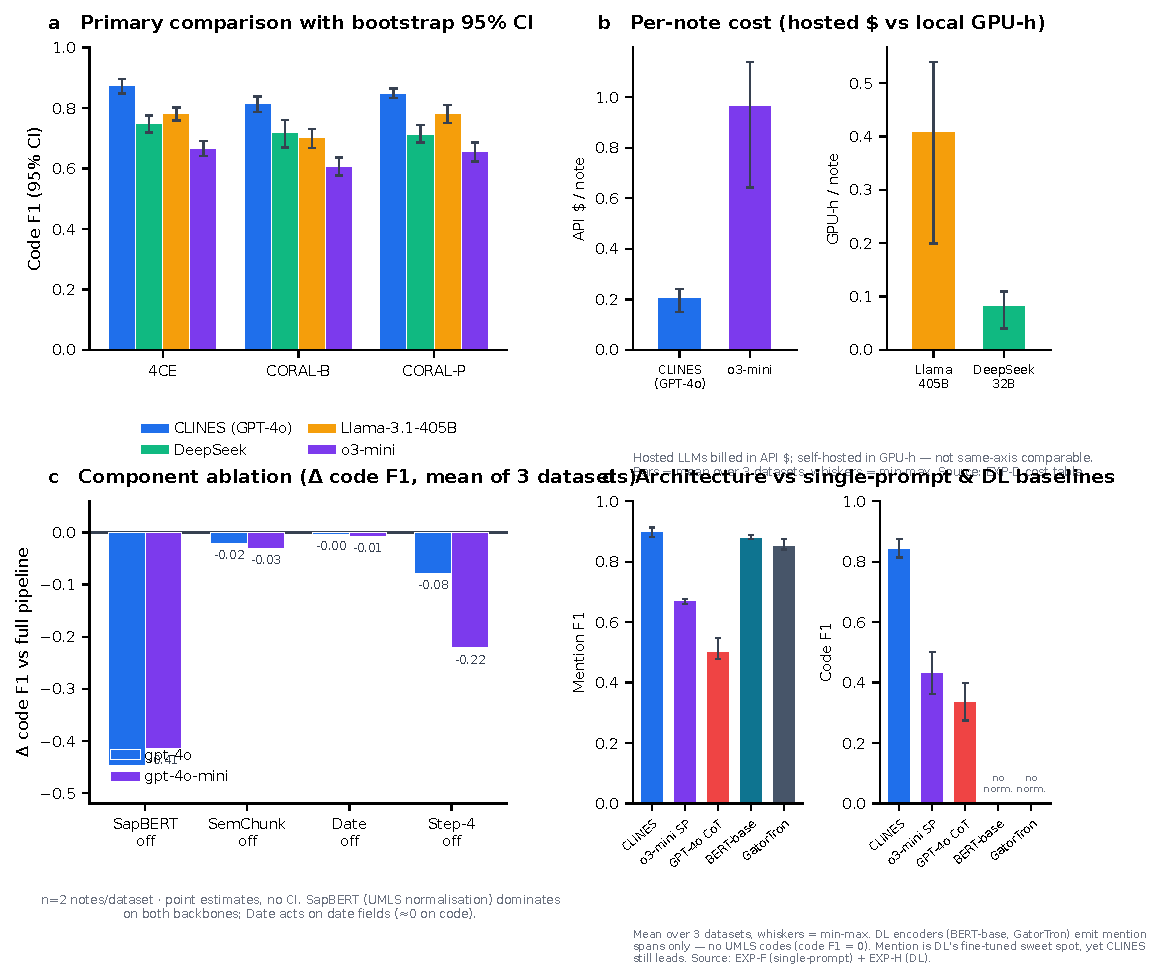
\includegraphics[width=\linewidth]{figures/figure5.pdf}
  \caption{\new{\textbf{Robustness, cost, and component contributions.} (a)~Primary CLINES (GPT-4o) code-F1 comparison against backbone alternatives with 95\% percentile bootstrap confidence intervals. (b)~Per-note cost: hosted-API dollars per note (CLINES (GPT-4o) versus o3-mini) and local GPU-hours per note (Llama-3.1-405B FP8 on 8$\times$H100); the dollar and GPU-hour axes are not directly comparable. (c)~Component ablation (change in code F1 relative to the full pipeline, mean of three datasets) for two backbones (GPT-4o and GPT-4o-mini); removing SapBERT-based UMLS normalization dominates on both backbones. (d)~CLINES versus single-prompt LLM baselines (o3-mini single-prompt, GPT-4o chain-of-thought) and full-size clinical deep-learning encoders (BERT-base clinical NER, GatorTron-base); the encoders emit entity spans only and produce no UMLS codes, so their code F1 is undefined.}}
  \label{fig:robustness-cost}
\end{figure}
